\chapter{Framework web}

\section{Motivations}
\textit{Construction d'un framework d'interface web sur la base des signaux introduits précédemment.}

\textit{Développement spécifiquement pour Scala.js. Il existe de nombreux bindings par exemple pour React ou Angular en Scala.js, mais l'utilisation d'un framework conçu pour JavaScript en Scala.js n'est pas toujours l'expérience la plus agréable. Volonté de disposer d'une API conçue pour le langage Scala.}

\section{Spécifications} \label{sec:web-specs}

\textit{L'architecture du framework web est encore à un stade très primitif.}

\subsubsection{Notation abrégée des packages}
Dans la suite de cette section, afin de réduire la longueur des noms des packages, une notation abrégée est utilisée à la place du nom complet d'une classe:
\begin{itemize}
	\item Le prefix \texttt{xuen} est abrégé en \texttt{x}.
	\item De façon similaire, le second niveau est abrégé en une seule lettre.
	\begin{itemize}
		\item \texttt{component} devient \texttt{c},
		\item \texttt{expression} devient \texttt{e},
		\item \texttt{template} devient \texttt{t},
		\item etc.
	\end{itemize}
\end{itemize}
Ainsi, par exemple, la classe \texttt{xuen.component.Element} est référencée par \texttt{x.c.Element}.

\subsection{Composant} \label{sec:web-usage-component}

Un composant est la brique essentiel de construction d'une application. Il correspond directement à une définition d'un \emph{custom element}. Une fois défini, un composant peut être instancié un nombre quelconque de fois, selon les besoins de l'application.

Un composant est défini à partir de:
\begin{itemize}
	\item Un sélecteur: correspondant à la balise HTML qui sera définie pour ce composant. Ce nom doit comporter un tiret (selon la spécification \emph{Custom Elements})
	\item Une implémentation: une sous-classe de \texttt{x.c.Element}, définissant le comportement des instances de ce composant
\end{itemize}
Optionnellement, un composant peut également posséder:
\begin{itemize}
	\item Un template: une structure HTML pouvant contenir des expressions de \emph{data-binding} avec des données réactives sous la forme de signaux, ce template sera matérialisé pour chaque instance du composant 
	\item Une feuille de styles: pouvant être utilisée pour définir l'apparence visuelle du composant
	\item Une liste de dépendances: une liste d'autres composants devant être chargés avant ce composant, cette liste correspond à d'autres composants utilisés dans le template de ce composant.
\end{itemize}

\subsubsection{Déclaration}
En pratique, un composant est créé en déclarant un \texttt{object} qui étend la classe \texttt{x.c.Component}. La classe correspondant à l'implémentation du composant est généralement déclarée simultanément avec le même nom, formant ainsi une paire (classe, objet compagnon) fréquent en Scala.

\begin{lstlisting}
import xuen.component._

class HelloWorld extends Element(HelloWorld)

object HelloWorld extends Component[HelloWorld](
	selector = "hello-world",
	template = html"""
		Hello, world!
	""",
	stylesheet = css"""
		:host { color: blue; }
	"""
)
\end{lstlisting}

Ce court exemple illustre déjà la plupart des concepts utilisés dans la construction de composants Xuen.

\subsubsection{Interpolateurs \texttt{html} et \texttt{css}}

Lors de la définition du template et de la feuille de style d'un composant, les interpolateurs \texttt{html} et \texttt{css} sont généralement utilisés. Ils sont une façon simple d'obtenir les objets de type \texttt{Template} et \texttt{Stylesheet} attendu par le constructeur de \texttt{Component} à partir de code source HTML ou CSS.

Ces interpolateurs sont définis par la classe \texttt{x.c.Interpolations}. En Scala, l'implémentation de tels interpolateurs repose sur l'utilisation de conversions implicites qui ne sont généralement pas identifiées automatiquement par l'IDE. Il est ainsi nécessaire d'importer cette classe manuellement afin de les utiliser. Alternativement, il est possible d'importer l'ensemble du package \texttt{xuen.component} en utilisant une importation \texttt{wildcard}.
\begin{lstlisting}
import xuen.component._
\end{lstlisting}
Cette méthode est généralement préférée à l'importation explicite.

Le nom d'interpolateur est trompeur: contrairement à l'interpolateur \texttt{s} de la bibliothèque Scala, \texttt{html} et \texttt{css} ne supporte pas l'insertion de fragments à l'aide du symbole spécial \texttt{\$}. Ils sont cependant une façon concise d'appliquer un traitement à une chaîne de caractères, en l'occurrence la transformation en instance de \texttt{Template} ou \texttt{Stylesheet}. Ils sont également l'occasion pour l'IDE d'identifier le langage utilisé dans la chaîne de caractères et ainsi offrir une coloration syntaxique et une auto-complétion appropriée.

Dans le cas d'IntelliJ IDEA, il est possible d'associer des langages arbitraires avec un interpolateur. Il est ainsi possible d'associer l'interpolateur \texttt{html} avec le langage HTML, de même pour \texttt{css} avec CSS. Dès lors, le code du template ou de la feuille de style sera correctement traité comme HTML ou CSS dans l'éditeur.

\subsubsection{Enregistrement et instantiation}

L'enregistrement du composant en tant que \emph{custom element} au niveau du navigateur se fait automatiquement lors de la construction de l'objet singleton \texttt{x.c.Component} de ce composant.

En Scala, la construction d'un \texttt{object} est différée jusqu'à la première référence de cet élément dans le code source, de façon similaire à l'initialisation d'une \texttt{lazy val}. La simple présence de la définition dans le code source n'est donc pas suffisante pour que ce composant soit enregistré. La méthode par laquelle le composant est instancié est alors importante.

Un composant peut être instancié de 4 façons différentes:
\begin{enumerate}
	\item Par l'utilisation du constructeur de son implémentation:
	\begin{lstlisting}
val element = new HelloWorld
	\end{lstlisting}
	\item En utilisant la méthode \texttt{instantiate} de \texttt{Component}:
	\begin{lstlisting}
val element = HelloWorld.instantiate()
	\end{lstlisting}
	\item En utilisant la méthode \texttt{createElement} de \texttt{Document}:
	\begin{lstlisting}
val element = dom.document.createElement("hello-world")
	\end{lstlisting}
	\item Implicitement par le parser HTML:
	\begin{lstlisting}
val div = dom.document.createElement("div")
div.innerHTML = "<hello-world></hello-world>"
	\end{lstlisting}
\end{enumerate}

Dans les deux premiers cas, l'objet \texttt{Component} est référencé directement ou indirectement et il n'est pas nécessaire de se préoccuper de l'enregistrement. Ce sont les méthodes préférées lorsque le composant est instancié par le code du développeur et non le navigateur lui-même.

Les deux autre méthodes se basent sur l'API native du navigateur et ne référencent à aucun moment l'objet \texttt{Component}. Ces méthodes n'enregistrent ainsi pas le composant au niveau du navigateur. Dans une telle situation, la fonction \texttt{Component.register} peut être utilisée pour forcer une référence vers l'objet \texttt{Component}. Un nombre arbitraire de composant peuvent être passés à \texttt{register}.
\begin{lstlisting}
Component.register(HelloWorld, AnotherComponent, ...)
\end{lstlisting}

Dans le cas des composants utilisés dans le template d'un autre composant, ces composants doivent être explicitement spécifiés dans la liste de dépendances du composant de premier niveau. Ainsi, référencer l'objet \texttt{Component} de niveau supérieur référencera également tous les composants des niveaux inférieurs et les enregistrement seront correctement effectués.
\begin{lstlisting}
object HelloWorld extends Component[HelloWorld](
	...,
	dependencies = List(One, Two, Three)
)
\end{lstlisting}

\subsection{Element} \label{sec:web-specs-element}

La définition du comportement d'un composant se fait par la définition d'une sous-classe de \texttt{x.c.Element} qui est ensuite passée au constructeur de \texttt{Component} (§ \ref{sec:web-usage-component}). Chaque instance du composant sera alors une instance de cette classe.

Un élément hérite de tous les éléments nécessaires à la définition d'un comportement de composant par le biais de la classe \texttt{x.c.Element}. Le seul paramètre restant à spécifier est le composant qui est implémenté par cet élément, ce qui est effectué par la paramètre passé au constructeur de \texttt{Element}.
\begin{lstlisting}
class HelloWorld extends Element(component = HelloWorld)
\end{lstlisting}

La déclaration ci-dessus est donc suffisante pour la définition d'un comportement de composant valide. La classe \texttt{Element} offre de nombreux outils aux instances de ses sous-classes.

\subsubsection{Interface \texttt{HTMLElement}}
\texttt{Element} hérite de l'interface \texttt{HTMLElement}, définie par le navigateur et les standards web. Cette interface hérite à son tour d'un ensemble d'autres interfaces tels que \texttt{dom.Element}\footnote{La spécification DOM défini également une interface \texttt{Element}, à distinguer de la classe abstraite \texttt{xuen.component.Element} qui est une implémentation spécifique de cette interface. En pratique, l'interface \texttt{x.c.Element} est rarement utilisée par le code utilisateur, et l'interface DOM est généralement utilisée en tant que \texttt{dom.Element} en Scala.js}, \texttt{dom.Node}, \texttt{EventTarget}.

Une instance de \texttt{Element} possède donc les méthodes et attributs usuels des éléments HTML, tel que par exemple \texttt{style}, \texttt{parentNode}, \texttt{querySelector} ou \texttt{addEventListener}. C'est aussi un argument valide pour les méthodes de manipulation du DOM tel que \texttt{appendChild} ou \texttt{replaceChild}.

\subsubsection{ShadowRoot}
Xuen se base sur les mécanismes du \emph{Shadow DOM} pour implémenter templates et feuilles de styles. Chaque instance d'un composant est ainsi associée à un sous-arbre Shadow DOM, accessible depuis l'attribut \texttt{shadow} définie par la classe \texttt{Element}.

Cet attribut est similaire à l'attribut \texttt{shadowRoot} définie par la spécification Shadow DOM à la différence que \texttt{shadow} est garanti d'être non-nul. Un sous-arbre Shadow DOM est automatiquement construit lors de l'accès à l'attribut si celui-ci n'existe pas. Un sous-arbre Shadow DOM est également automatiquement construit si le composant a défini un template ou une feuille de style et sera initialement peuplé par les éléments correspondants.

Il est généralement déconseillé de manipuler le sous-arbre Shadow DOM manuellement. Ceci est en général effectué de façon déclarative à partir du template. Il peut cependant être nécessaire d'accéder à l'instance d'un élément présent dans le sous arbre à partir de l'implémentation du composant. Dans une telle situation \texttt{querySelector} peut être utilisé à partir de \texttt{shadow} pour accéder aux éléments du sous-arbre.

\begin{lstlisting}
class HelloWorld extends Element(HelloWorld) {
	private val span = shadow.querySelector("span")
	span.addEventListener("click", ...)
}

object HelloWorld extends Component[HelloWorld](
	selector = "hello-world",
	template = html"""Hello, <span>world</span>!"""
)
\end{lstlisting}

À noter que, conformément à la spécification Shadow DOM, invoquer la méthode \texttt{querySelector} directement sur l'instance \texttt{Element} ne permet pas d'accéder aux éléments du sous-arbre Shadow DOM, uniquement aux enfants hors du sous-arbre caché, appelé \emph{light DOM}.

\begin{lstlisting}
// Instancié à partir de :
// <hello-world><span>a</span></hello-world>

class HelloWorld extends Element(HelloWorld) {
	private val a = this.querySelector("span")
	private val b = this.shadow.querySelector("span")
	assert(a.textContent == "a")
	assert(b.textContent == "b")
}

object HelloWorld extends Component[HelloWorld](
	selector = "hello-world",
	template = html"""<span>b</span>"""
)
\end{lstlisting}

\subsubsection{Attributs}
Les attributs jouent un rôle similaire aux arguments de constructeur en HTML, ils sont un mécanisme permettant de passer des paramètres à un élément afin de configurer son comportement.

Un élément Xuen peut définir un ensemble de paramètre auxquels il souhaite avoir accès sous forme d'un signal \texttt{Source}. La valeur de l'attribut sera reflétée dans le signal correspondant. Cette association est \emph{live}, c'est à dire que l'attribut sera automatiquement observé et la valeur du signal sera mise à jour si un événement externe venait à modifier sa valeur. Inversement, un changement de la valeur de la source entraînera automatiquement une mise à jour de l'attribut HTML correspondant.

Un \emph{binding} d'attribut est déclaré en utilisant la méthode \texttt{attribute[T]}, produisant un \texttt{Source} de type \texttt{T} pour l'attribut. Le nom de l'attribut est automatiquement déterminé en fonction du nom de la variable à laquelle cette source est associée.

\begin{lstlisting}
class HelloWorld extends Element(HelloWorld) {
	val foo = attribute[String]
	// Association avec l'attribute `foo`
}
\end{lstlisting}

Si la détection automatique ne parvient pas à identifier automatiquement le nom de l'attribut en question, une erreur sera générée à la compilation. Il est alors possible de spécifier explicitement le nom de l'attribut. Ceci permet également d'associer un nom différent à la source et à l'attribut manipulé.

\begin{lstlisting}
class HelloWorld extends Element(HelloWorld) {
	val bar = attribute[String]("foo")
}
\end{lstlisting}

La valeur d'un attribut d'un élément HTML est toujours une chaîne de caractères. Un \emph{binding} d'attribut effectue automatiquement une sérialisation ou désérialisation entre la valeur effective de l'attribut de type \texttt{String} et le type \texttt{T} utilisé par le signal.

Cette opération nécessite qu'une instance du trait \texttt{x.c.AttributeFormat[T]} soit implicitement disponible pour le type \texttt{T} en question. Par défaut, les types \texttt{String}, \texttt{Boolean}, \texttt{Char}, \texttt{Byte}, \texttt{Short}, \texttt{Int}, \texttt{Long}, \texttt{Float} et \texttt{Double} peuvent être utilisés pour un attribut.

\subsubsection{Propriétés}
Les propriétés sont une alternative aux attributs qui ne dépendent pas de \texttt{AttributFormat} et peuvent donc être utilisés pour passer n'importe quel type de paramètre à un élément Xuen. 

\begin{lstlisting}
class HelloWorld extends Element(HelloWorld) {
	val foo = property[Map[Int, String]]
}
\end{lstlisting}

En pratique, une déclaration \texttt{property[T]} correspond à la construction d'une \texttt{Source.undefined[T]}. Cependant, l'usage de \texttt{property} souligne l'usage attendu de la source en tant que paramètre de l'élément.

\subsubsection{Événements personnalisés}

\textit{Méthodes simplifiée pour le traitement d'événement personnalisés dans un Element.}

\subsubsection{Événements \texttt{xuen:connected} et \texttt{xuen:disconnected}}

\textit{Custom events lors de la connexion / déconnexion d'un élément}

\subsection{Template}

Un template est une structure de noeuds DOM qui sont automatiquement insérés dans le sous-arbre Shadow DOM d'un composant lorsque celui-ci est instancié. Cette structure est généralement définie à partir du code source HTML correspondant et l'interpolateur \texttt{html}, en paramètre au constructeur de \texttt{Component}.

Cette structure est \emph{compilée} lors de la création de l'objet correspondant \texttt{Template}. Le compilateur va ainsi parcourir récursivement la structure originale afin d'identifier des annotations de \emph{data-binding} associant des comportements particuliers à certains noeuds de l'arbre.

Ces annotations sont fortement inspirées de la syntaxe utilisée par le framework \emph{Angular 2} et prennent la forme d'attributs particuliers placés sur les éléments du template. La comportement exact de ces annotations est spécifié par l'\emph{expression} utilisée comme valeur de l'attribut. La section \ref{sec:web-usage-expr} détail spécifiquement la syntaxe des expressions. Cette section se concentre sur les annotations disponibles.

\subsubsection{Interpolation}
Les noeuds \texttt{Text} et les attributs d'éléments présents dans le template peuvent contenir des marqueurs d'interpolation \texttt{\{\{ \}\}}. L'expression contenue dans la double-paire d'accolade sera évaluée puis convertie en \texttt{String} avant d'être insérée à la place du marqueur dans le texte final.

\begin{lstlisting}[language=HTML]
<div>2 + 2 = {{ 2 + 2 }}</div>
--> <div>2 + 2 = 4</div>

<canvas width="720" height="{{9/16 * 720}}"></canvas>
--> <canvas width="720" height="405"></canvas>
\end{lstlisting}

Une expression d'interpolation ne peut jamais échouer, les cas de valeurs \texttt{null} et \texttt{undefined} sont explicitement gérés en retournant le texte correspondant. Dans tous les autres cas, la méthode \texttt{toString} est utilisée pour produire la valeur finale.

Il n'est pas possible de placer une interpolation dans un attribut dont le contenu est déjà interprété comme une expression. C'est par exemple le cas des attributs qui sont des annotations de \emph{data-binding}. Il n'est pas non plus possible d'emboîter une interpolation dans une autre.

Il est cependant autorisé de placer une interpolation dans un commentaire HTML comme utilitaire de développement.

\subsubsection{Annotation d'identifiant}
Un attribut dont le nom débute par \texttt{\#} est traité comme une annotation d'identifiant, spécifiant la valeur de l'attribut \texttt{id} de l'élément. Cette simple annotation est principalement un sucre syntaxique et la valeur de l'attribut, si elle est spécifiée, est ignorée.

\begin{lstlisting}[language=HTML]
<div #foo></div>
--> <div id="foo"></div>
\end{lstlisting}

\subsubsection{Annotation de classe}
Un attribut dont le nom commence par \texttt{.} est traité comme une annotation de classe. Si aucune valeur n'est fournie pour cet attribut, la classe est inconditionnellement ajoutée aux classes de l'élément.

Si une valeur est fournie pour cet attribut, celle-ci évaluée en tant qu'expression booléenne. Si la valeur évaluée est \texttt{true}, la classe est ajoutée à la liste de classes de l'élément. Dans le contraire, la classe est retirée de l'élément. Si cette expression utilise des signaux, ce comportement est dynamique et la classe correspondante sera ajoutée ou retirée au fil du temps.

\begin{lstlisting}[language=HTML]
<div .foo .bar="true" .baz="false"></div>
--> <div class="foo bar"></div>
\end{lstlisting}

\subsubsection{Annotation de propriété}
Un attribut dont le nom commence par \texttt{[} et se termine par \texttt{]} est traité comme une annotation d'attribut.

La valeur de l'attribut est évaluée en tant qu'expression et la valeur obtenue est utilisée pour mettre à jour la propriété correspondante de l'élément. Si cette propriété est une \texttt{Source}, la valeur de la source est modifiée à la place.

\begin{lstlisting}[language=HTML]
<input type="text" [value]="2 + 2">
--> <input type="text"> == $0
--> $0.value == "4"
\end{lstlisting}

Il est important de souligner que ce type d'annotation n'affecte pas les \emph{attributs} de l'élément mais bien les \emph{propriétés} de l'objet JavaScript correspondant. C'est pourquoi dans l'exemple ci-dessus il n'y a pas d'attribut \texttt{value} présent sur l'élément \texttt{<input>}, mais \texttt{\$0.value} retourne effectivement la chaîne de caractères \texttt{"4"}\footnote{La notation \texttt{\$0} est inspirée de l'inspecteur web de Google Chrome, dans lequel la variable \texttt{\$0} fait référence à l'élément actuellement sélectionner dans l'inspecteur DOM.}.

Si aucune valeur n'est fournie pour l'annotation de propriété, la nom de la propriété est utilisée comme expression. Ainsi, une annotation \texttt{[foo]} est traitée en tant que \texttt{[foo]="foo"}, offrant ainsi une syntaxe raccourcie dans le cas où une propriété d'un élément parent est passée tel quel à une propriété du même nom dans un élément enfant.

\subsubsection{Annotation d'événement}

Un attribut dont le nom commence par \texttt{(} et se termine par \texttt{)} est traité comme une annotation d'événement.

La valeur de l'attribut sera évaluée à chaque fois que l'événement correspondant sera \emph{dispatché} à partir de l'élément. À l'intérieur de cette expression, la variable \texttt{event} fait référence à l'instance de l'événement émis. Il est interdit de ne pas spécifier de valeur pour une annotation d'événement.

\begin{lstlisting}[language=HTML]
<input type="text" (input)="doSomethingWith(event.target.value)">
\end{lstlisting}

Les événements sont écoutés sur l'élément annoté, et du point de vue de l'élément parent. En d'autre termes, le gestionnaire d'événement est attaché à l'élément lui-même, il n'y a donc pas besoin que l'élément se propage dans l'arbre DOM pour être reçu. En revanche, si l'élément provient du sous-arbre Shadow DOM de l'élément, il est possible qu'il ne traverse pas la barrière du Shadow DOM et soit ainsi invisible à partir de l'élément parent.

Un certains nombre d'événements traversent naturellement la barrière du Shadow DOM, c'est la cas par exemple de \texttt{click}, \texttt{input} ou \texttt{mousemove}. D'autres, comme par exemple tous les événements personnalisés, sont par défaut encapsulés dans le sous-arbre et invisibles de l'extérieur de l'élément. Un tel événement ne pourra être capturé par cette annotation. Dans le cas d'un événement personnalisé, il est nécessaire que le flag \texttt{composed} soit défini à \texttt{true} lors de la création de l'événement.

\subsubsection{Transformation \texttt{*if}}
Une transformation est une annotation qui modifie dynamiquement la structure du DOM à partir d'expressions.

La transformation \texttt{*if} évalue sa valeur en tant qu'expression booléenne. Si la valeur obtenue est \texttt{true}, l'élément est inséré dans l'arbre DOM. Si la valeur est \texttt{false}, l'élément est retiré de l'arbre et un commentaire est inséré à la place en tant que \emph{placeholder}.

\begin{lstlisting}[language=HTML]
<div> <div *if="true"></div> </div>
--> <div> <div></div> </div>

<div> <div *if="false"></div> </div>
--> <div> <!-- *if false --> </div>
\end{lstlisting}

\subsubsection{Transformation \texttt{*for}}
La valeur de la transformation \texttt{*for} doit être un \texttt{énumérateur}, une expression particulière définissant les différentes propriétés de l'itération. Pour chaque élément de l'énumérateur, l'élément sera dupliqué et inséré dans l'arbre DOM.

À l'intérieur d'un élément annoté avec \texttt{*for}, les variables déclarées par l'énumérateur sont accessibles et correspondent à la valeur courante de l'itération. Il est également possible d'utiliser ces variables pour d'autres annotations présentes sur l'élément, les transformations étant appliquées avant les annotations.

\begin{lstlisting}[language=HTML]
<ul> <li *for="i of [1, 2, 3]">{{i}}</li> </ul>
--> <ul> <li>1</li> <li>2</li> <li>3</li> </ul>
\end{lstlisting}

\subsubsection{Précédence des transformations}
Si les transformation \texttt{*if} et \texttt{*for} sont simultanément présentes sur un élément, la transformation \texttt{*if} est appliquée en premier, suivi de la transformation \texttt{*for}.

L'objectif est d'offrir un mécanisme permettant la désactivation conditionnelle de l'ensemble de l'itération, en traitant \texttt{*if} avant \texttt{*for}, plutôt que l'élision d'un élément particulier de l'itération, ce qui se produirait si \texttt{*for} était évalué avant \texttt{*if}. En effet la clause de filtrage \texttt{if} de l'énumérateur offre déjà ce mécanisme.

\subsubsection{Utilisation combinée des transformations avec \texttt{<template>}}
Du fait de la syntaxe du langage HTML, il n'est possible d'appliquer une annotation que sur un élément, et non un noeud DOM quelconque. Il n'est par exemple pas possible d'annoter un noeud \texttt{Text}.

Dans le cas des annotations basiques, cela n'a généralement pas d'importance, un noeud \texttt{Text} ne possède de toutes façons pas d'attribut \texttt{id}, \texttt{class} ou de propriétés particulières. Il n'émet pas non plus d'événements. Cependant, dans le cas des annotations de transformations, l'impossibilité d'annoter un noeud \texttt{Text} peut se révéler gênant.

\begin{lstlisting}[language=HTML]
<div><span>...</span> ??*if="..."??text <span>...</span></div>
--> Nothing to put the `*if` on ?!
\end{lstlisting}

Au autre situation problématique est l'annotation simultanée de plusieurs éléments. Comment faire lorsque une transformation \texttt{*for} doit produire deux éléments DOM pour chaque élément de l'itération ? Dans l'exemple ci-dessous, chaque \emph{checkbox} est associée à un label.

\begin{lstlisting}[language=HTML]
<input *for="i of [1, 2]" type="checkbox" [value]="i">
<span *for="i of [1, 2]">{{i}}</span>
\end{lstlisting}

Cet exemple produit une liste de 3 \emph{checkboxes} puis 3 labels, certainement pas le résultat escompté.

Une solution serait d'encapsuler les noeuds à annoter dans une élément neutre tel que \texttt{<div>} ou \texttt{<span>} et d'annoter cet élément. Cette solution est relativement simple et est généralement la méthode préférée dans ce genre de situation.

Cependant, l'ajout d'un élément supplémentaire peut avoir des effets secondaires indésirables, par exemple au niveau des sélecteurs CSS. Dans le cas d'une itération, ceci n'est pas toujours possible. Dans ces situations, il est possible d'utiliser un élément \texttt{<template>} afin d'encapsuler un nombre quelconque de sous-noeuds DOM.

\begin{lstlisting}[language=HTML]
<template *for="i of [1, 2]">
	<input type="checkbox" [value]="i">
	<span>{{i}}</span>
</template>
\end{lstlisting}

Lorsqu'une transformation est appliquée sur un élément \texttt{<template>}, cet élément est supprimé du sous-arbre DOM produit par la transformation et seul son contenu est inséré. Il se substitue ainsi à l'élément encapsulant mentionné précédemment et disparait totalement lors de l'application de la transformation.

\subsection{Expressions} \label{sec:web-usage-expr}
Les expressions sont à la base des comportements dynamiques dans les templates Xuen. Elles sont fortement inspirées de la syntaxe de JavaScript et suivent en grande partie la sémantique de celui-ci.

Les expressions sont conçues pour être utilisées en combinaison avec les signaux Xuen. Le résultat de l'évaluation d'une expression est transformé en \texttt{Signal}, permettant ainsi de profiter du mécanisme de propagation des changements implémentés dans les signaux. Lorsqu'un signal référencé dans une expression change, la valeur de l'expression est recalculée et le template mis à jour en conséquence.

À l'intérieur même d'une expression, les signaux accédés sont décomposés par l'interpréteur. Si l'interpréteur rencontre un fragment d'expression produisant une valeur de type \texttt{Signal[T]}, cette valeur sera transformée en simple \texttt{T} en invoquant la méthode \texttt{value} du signal. Ce processus est récursif, une valeur de type \texttt{Signal[Signal[T]]} sera également extraite en une valeur \texttt{T}. Si un signal indéfini est rencontré, la valeur \texttt{undefined} est utilisée à la place. L'évaluation de l'expression continue alors avec la nouvelle valeur.

Il n'est donc pas nécessaire lors de la construction d'une expression de se soucier de l'encapsulation d'une valeur dans un signal puisque celui-ci sera automatiquement retiré par l'interpréteur.

\begin{figure}[h]
	\begin{lstlisting}
class HelloWorld extends Element(HelloWorld) {
	val name = attribute[String]
	// `name` est une `Source[String]` une sous-classe de `Signal[String]`
}

object HelloWorld extends Component[HelloWorld](
	selector = "hello-world",
	template = html"""
		Hello, {{name}}!
		<!-- Dans une expression, `name` est traité comme une simple valeur `String` -->
	"""
)

// Utilisation:
<hello-world name="Bastien"></hello-world>
	\end{lstlisting}
	\caption{Exemple illustrant l'extraction automatique des valeurs \texttt{Signal} lors de l'évaluation d'une expression}
\end{figure}

\subsubsection{Contexte d'évaluation}
Une expression est toujours évaluée par rapport à un contexte spécifique. Ce contexte défini le monde extérieur autour de l'expression. Il est pas exemple utilisé lorsque l'expression fait référence à des variables ou des fonctions. Dans ce cas, le contexte est invoqué pour obtenir la valeur de cette variable.

Dans la plupart des cas, le contexte d'une expression sera l'\texttt{Element} auquel le template est associé. Les variables et les fonctions invoquées correspondent respectivement aux propriétés et méthodes de l'objet \texttt{Element}.

\begin{lstlisting}
class HelloWorld extends Element(HelloWorld) {
	val foo = 2
	def bar(v: Int): Int = v * 3
}

<div>{{ foo + bar(5) }}</div>
--> <div>17</div>
\end{lstlisting}

Certaines constructions, par exemple une transformation \texttt{*for} ou une annotation d'événement, peuvent introduire des contextes \emph{enfants}. Ces contextes sont comparables au concept de \emph{scope} d'un langage de programmation. Les propriétés présentes sur le contexte enfant sont disponibles en plus des propriétés du contexte parent. Dans le cas où une propriété est présente à la fois dans le contexte parent et le contexte enfant, la propriété du contexte enfant masque celle du contexte parent (\emph{shadowing}).

\begin{lstlisting}
class HelloWorld extends Element(HelloWorld) {
	val foo = List(3, 5)
	val i = 8
	val j = 13
}

<div>
	<span>{{i + j}}</span>
	<span *for="i of foo">{{i + j}}</span>
</div>
--> <span>21</span> <span>16</span> <span>18</span>
\end{lstlisting}

\subsubsection{Opérateur d'accès protégé \texttt{?.}}
L'opérateur \texttt{?.} est similaire à l'usage à l'opérateur simple \texttt{.}: il permet d'accéder à une propriété ou une méthode de l'expression à sa gauche et prend un identifier à sa droite pour identifier la propriété accédée.

En revanche, lorsque l'expression à gauche de l'opérateur \texttt{.} est \texttt{undefined}, tenter de l'indexer avec l'opérateur \texttt{.} provoque une erreur. Ceci est utile en phase de développement pour identifier les situations où une référence qui ne devrait pas être indéfinie l'est tout de même.

Dans le cas où il est normale que le membre de gauche puisse être \texttt{undefined}, l'usage de l'opérateur protégé \texttt{?.} ne provoque pas d'erreur et retourne simplement \texttt{undefined} à son tour, permettant ainsi de le chaîner autant de fois que nécessaire. Si la référence indexée est définie, l'opérateur \texttt{?.} se comporte de façon identique à l'opérateur \texttt{.} classique.

\subsection{Feuille de styles}
La feuille de styles d'un composant est un simple fragment de code CSS qui sera injecté dans le sous-arbre Shadow DOM d'un composant. Aucun traitement particulier n'est appliqué au code source CSS.

La feuille de styles est injectée sous la forme d'un élément \texttt{<style>} contentant les définitions CSS. Puisque cet élément est placé dans un sous-arbre DOM, la portée de ses sélecteurs est limitée à ce sous-arbre. Il n'y a donc pas de conflits au niveau des identifiant des éléments du template (attribut \texttt{id}) ou du nom des classes, conduisant à des sélecteur extrêmement simples et concis.

Spécifiquement l'élément \texttt{<style>} est inséré en tant que dernier enfant du sous-arbre Shadow DOM. Ce qui a pour implication que le dernier élément du template ne vérifie pas le sélecteur \texttt{:last-child}, puisque l'élément \texttt{<style>} est en pratique le dernier élément du template. En revanche, le sélecteur \texttt{:first-child} identifie correctement le premier élément dans le template. Si l'usage du sélecteur \texttt{:last-child} s'impose, il est possible d'envelopper le template dans un élément \emph{wrapper} et ainsi ignorer la présence de l'élément \texttt{<style>} en tant que dernier fils du sous-arbre.

Il est possible de faire référence à l'élément hôte lui même, c'est à dire l'élément possédant la racine du sous-arbre Shadow DOM, avec le sélecteur \texttt{:host}. La version fonctionnelle de ce sélecteur (\texttt{:host(selector)}) permet de faire référence à l'élément hôte uniquement si celui-ci vérifie également le sélecteur passé en paramètre.

L'élément sélectionné par le sélecteur \texttt{:host} correspond à l'élément personnalisé lui-même, qui est également accessible en dehors du sous-arbre Shadow DOM. Dans le cas où une propriété CSS est définie à la fois à l'intérieur (par la feuille de styles de l'élément lui-même) et à l'extérieur du sous-arbre Shadow DOM (par une feuille de styles dans le contexte parent), la définition extérieur s'applique et la définition intérieur est ignorée. Par exemple, la marge interne d'un élément \texttt{<hello-world>} dont la feuille de styles contiendrait \texttt{:host \{ padding: 12px; \}} pourrait être modifiée en spécifiant: \texttt{hello-world \{ padding: 0px; \}} dans la feuille de styles de l'élément parent (ou du document).

Ces sélecteurs ne sont pas une spécificité de Xuen, ils font partie de la spécification \emph{CSS Scoping} des standards web. Puisque Xuen se base sur l'implémentation standard des \emph{Web Components} pour ses propres composants, il est possible de profiter des standards annexes développés pour \emph{Web Components} lorsque cela est applicable.

\subsubsection{Variables CSS}
Le mécanisme de variables CSS est également un standard web qui est à présent implémenté dans la quasi-totalité des navigateurs modernes. En pratique le support des variables CSS est plus répandu que le support de \emph{Shadow DOM} et \emph{Custom Elements}, elles peuvent donc être considérée comme utilisables dans ce projet.

Une variable CSS prend la forme d'une propriété personnalisée dont le nom débute par deux tiret \texttt{--}. Par exemple, la déclaration \texttt{--foo: 2} défini une variable \texttt{--foo} dont la valeur est \texttt{2}.

Le nom de \emph{variable} est trompeur. En pratique, ces constructions se comportent plus comme une constante, qui est propagée entre les éléments par le mécanisme de cascade classique de CSS. Cette valeur peut alors être redéfinie et la nouvelle valeur sera effective pour le reste de la cascade.

Ceci peut être comparé à la valeur de la propriété \texttt{font-size} qui est appliquée par cascade à tous les sous-élément de l'élément auquel elle est appliquée, et qui peut être écrasée par la définition d'une nouvelle propriété \texttt{font-size} sur l'un de ces sous-éléments.

La valeur d'une variable CSS est accédée par la fonction \texttt{var()} prenant le nom de la variable en paramètre et optionnellement une valeur par défaut. Par exemple,
\begin{lstlisting}[language=HTML]
body {
	--bg-color: blue;
}

div {
	background-color: var(--bg-color, red);
}
\end{lstlisting}

Les variables CSS sont la méthodes préférée pour paramétrer l'apparence d'un élément personnalisé. La liste des variables CSS utilisée par un élément sont ainsi une part intégrale de l'interface publique de l'élément.

\subsection{Service}

\subsection{Router}

\section{Solutions existantes}

\subsection{Bindings.scala et Monadic-HTML}

\emph{Bindings.scala} \cite{binding.scala} et \emph{Monadic-HTML} \cite{monadic-html} sont deux exemples d'implémentation d'un système de template basés sur les concepts de la programmation réactive-fonctionnelle.

Ces deux bibliothèques sont très similaires, \emph{Monadic-HTML} étant initialement inspirée de \emph{Bindings.scala}. Parmi les différences notables, on peut noter l'approche basée sur les macros compilateur utilisée par \emph{Bindings.scala} et la ré-implémentation des classes XML de Scala dans \emph{Monadic-HTML}.

Dans les deux cas, l'objectif est de transformer le code du développeur composé sur la base des littéraux XML intégrés au langage Scala en une structure dynamique qui peut être insérée dans l'arbre DOM du document.

Les littéraux XML, initialement ajoutés au langage Scala alors que l'usage de XML était beaucoup plus prévalent qu'il ne l'est aujourd'hui, sont aujourd'hui considéré comme une complexité excessive du langage et sont sur le point d'être retirés en faveur d'un interpolateur \texttt{xml}. Dans le cas de \emph{Bindings.scala}, l'implémentation sous forme de macros devra être ré-implémentée pour supporter la nouvelle syntaxe proposée.

Dans le cas de \emph{Monadic-HTML}, l'approche n'est tout simplement plus valide. La bibliothèque utilise en effet une implémentation alternative des classes XML utilisées par Scala pour matérialiser les littéraux XML à l'exécution, en principe disponibles dans une bibliothèque indépendante. Puisque la syntaxe n'est que sucre syntaxique au niveau du compilateur, les nouvelles classes dont la sémantique est considérablement différentes de l'implémentation originale sont utilisées aveuglément par le compilateur et conduisent au résultat désiré.

Le retrait du support de la syntaxe XML au niveau du compilateur Scala serait synonyme de retrait de l'implémentation des sugres syntaxiques sur lesquels  \emph{Monadic-HTML} est construit, sans offrir d'alternatives évidentes puisque le mécanisme était un \emph{hack} dès le début.

Dans le cadre du développement de Xuen, le choix a été fait de mettre de côté les littéraux XML, pour se concentrer sur une implémentation basée sur les interpolateurs. Par conséquent, une partie du travail précédemment effectué par le compilateur Scala au moment de la compilation est à présent effectué au \emph{runtime} dans le navigateur. La disponibilité du DOM et du parser HTML du navigateur est un avantage au niveau de l'implémentation, mais les performances s'en trouvent inévitablement impactées. L'approche n'exclut pas une utilisation future de macros pour effectuer la compilation du template au moment de la compilation du code.

Une autre différence notable entre ces bibliothèques et Xuen est le niveau d'encapsulation utilisé.  \emph{Monadic-HTML} et \emph{Bindings.scala} produisent des morceaux d'arbre DOM qui sont ensuite insérés dans le document, sans encapsulation particulière, notamment en ce qui concerne l'application de styles CSS. Xuen propose dès le départ une abstraction sous forme de \emph{composants} indépendants et isolés construit sur la base des derniers standards du web.

L'implémentation des signaux de ces deux bibliothèques diffère légèrement de l'implémentation qui en est fait dans Xuen. Les signaux sont manipulés explicitement de façon monadique , il n'existe pas de signaux pouvant représenter des expressions arbitraire. La notion de signaux indéfinis est également absente. Il est nécessaire d'encapsuler explicitement les données manipulées dans une instance de la classe \texttt{Option} si le signal peut potentiellement être indéfini, conduisant à une plus grand verbosité à l'utilisation.
\section{Implémentation}

\subsection{Vue d'ensemble}
\begin{figure}[h]
	\centering
	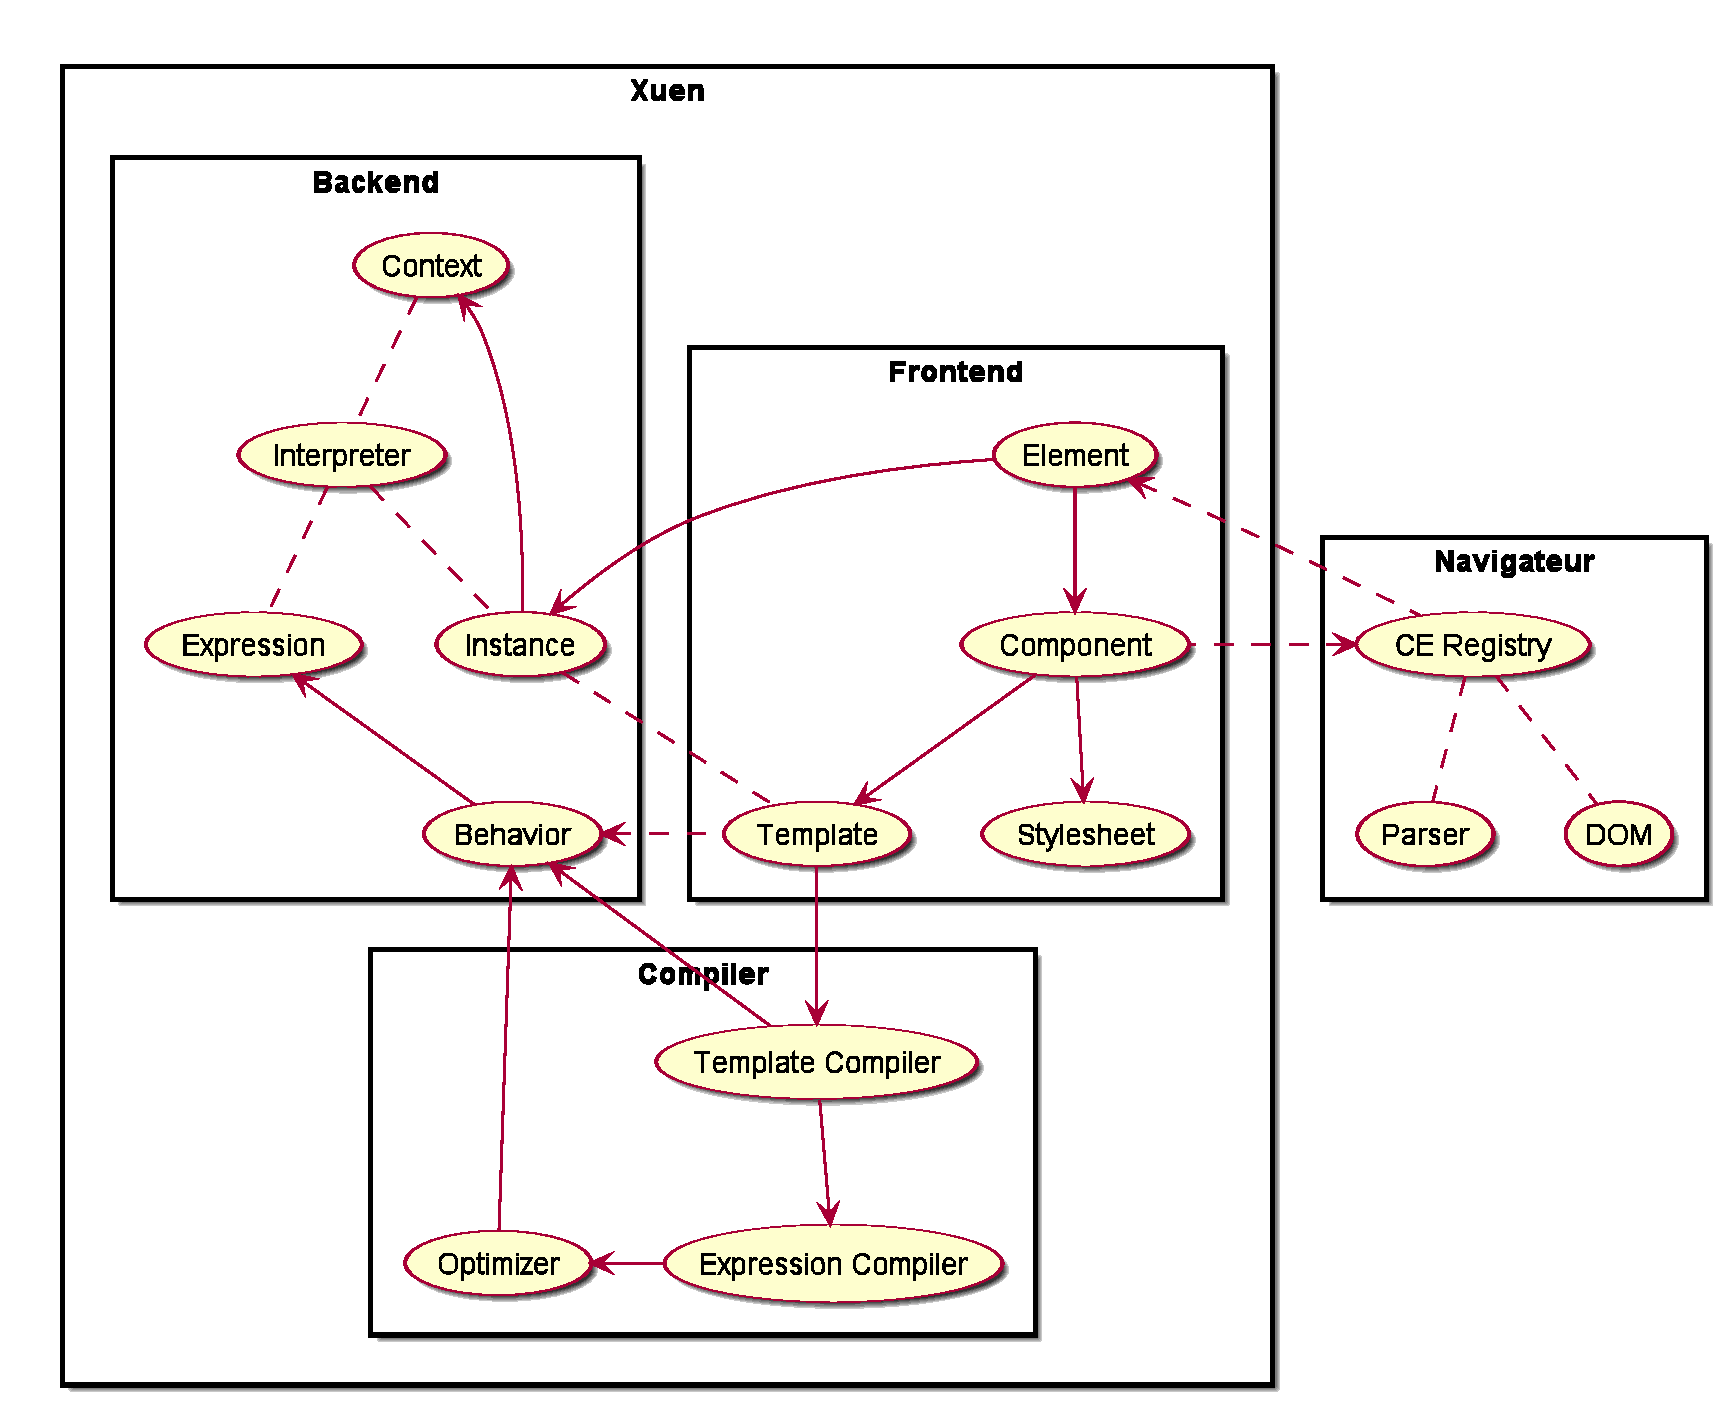
\includegraphics[width=\textwidth]{img/web_overview.eps}
	\caption{Vue d'ensemble de l'implémentation du framework Web}
	\label{fig:web-overview}
\end{figure}

L'implémentation du framework web de Xuen peut être décomposé en 3 grandes parties, tel qu'illustré par la figure \ref{fig:web-overview}.

\begin{enumerate}
	\item La partie \emph{front-end} est exposée directement au développeur. Elle est utilisée pour déclarer les composants personnalisés de l'application, leurs comportement et structure.
	\item La partie \emph{back-end} est utilisée par le framework lorsqu'un élément est instancié dans le document. Elle fournit les outils nécessaires à l'implémentation des comportements dynamiques du template de cet élément et l'interface avec le système de signaux par le biais des expressions.
	\item Finalement le système de compilation est utilisé lors de la définition d'un nouveau composant pour transformer le code source HTML du template en une instance de la classe \texttt{Template}, encapsulant à la fois une structure pré-traitée du template, des modèles pour construire les comportements dynamiques de ce template et des expressions sous forme d'arbres syntaxiques prêts à être interprétés.  
\end{enumerate}

L'objectif de la partie de compilation est de réduire l'impact du traitement du template au \emph{runtime}. En effet, l'instanciation d'un template se base sur les outils fournis par le navigateur, notamment le parser HTML et son implémentation du DOM afin parcourir et traiter la structure fournie sous forme de code HTML.

En compilant le template et les expressions dès la déclaration, il n'est plus nécessaire de le faire lors de l'instanciation, ce qui permet un investissement fixe au chargement de l'application et des performances accrues lors de son fonctionnement.

Cette structure est en grande partie reprise d'un projet personnel antérieur. La plupart des éléments ont été repensés et réimplémentés, principalement pour les adapter au nouveaux standards \emph{Web Components} version \emph{v1} (par opposition à la version antérieure \emph{v0}). Le parser d'expression a quant à lui été réécrit, passant d'une implémentation fortement inspirée du parser d'expression du framework Angular 2, mais en Scala, à une version développée avec la bibliothèque \emph{scala-parser-combinators} \cite{scala-parser-combinators}, plus propre et idiomatique. La grammaire du langage n'a cependant pas été significativement modifiée. L'optimisateur d'expressions est réutilisé pratiquement tel quel.

\subsection{Processus de compilation du template}

Le template est fourni à la bibliothèque sous forme de code source HTML. La première opération consiste donc à construire dynamiquement un élément \texttt{<template>} et à y insérer le code du développeur. Le parser HTML du navigateur sera alors invoqué pour construire une structure de nœuds DOM. Cette structure est ensuite parcourue de façon récursive en commençant à l'élément template créé précédemment.

\begin{itemize}
	\item Premièrement, la nature du noeud en cours est déterminée. S'il s'agit d'un nœud \texttt{Text} ou \texttt{Comment}, son contenu est scanné pour y identifier d'éventuelles interpolations.
	\item Si le nœud est un élément, ses attributs sont observés.
	\item Si l'élément est annoté d'une transformation \texttt{*if} ou \texttt{*for}, cette transformation est appliquée.
	\item Si l'élément possède des annotations de \emph{data-binding}, celles-ci sont traitées.
	\item Les valeurs des attributs restants qui ne sont ni des transformations ni des annotations de \emph{data-binding} sont scannées pour y identifier des interpolations.
	\item Une fois l'élément lui-même entièrement traité, l'ensemble de ses enfants est parcouru, réitérant le processus.
\end{itemize}

Pour chaque nœud DOM devant être associé à un comportement dynamique, un \texttt{Behavior} est créé. Celui-ci est identifié par un numéro incrémenté à chaque nouvelle instance. Il sera de modèle pour la construction du comportement dynamique en question. Tous les \texttt{Behavior}s créés pour un template son rassemblé dans une \texttt{Map} contenue dans l'objet \texttt{Template} resultant. L'élément auquel le comportement doit être attaché est quant à lui décoré d'un attribut \texttt{xuen:behavior="..."} indiquant l'identifiant du comportement associé à ce nœud.

Si l'élément ne peut pas posséder d'attribut, c'est à dire lorsqu'il s'agit d'un nœud \texttt{Text} ou \texttt{Comment}, un élément \emph{placeholder} \texttt{<xuen:placeholder>} est inséré à sa place dans l'arbre DOM du template et l'attribut est placé sur cet élément. Dans ce cas, lors de la construction du comportement au moment de l'instanciation du template, l'élément \emph{placeholder} sera en premier lieu remplacé par un nœud correspondant à l'original puis le comportement spécifique de ce nœud sera implémenté.

Un \texttt{Behavior} peut en réalité implémenter plus d'un comportement pour un même élément. Si deux annotations sont présentes sur un même élément, le \texttt{Behavior} construit à l'occasion du traitement de la première annotation est réutilisé pour la deuxième annotation. L'objet \texttt{Behavior} sera donc en charge de construire deux comportements dynamiques différents sur le même élément.

À l'inverse de la compilation, le processus d'instanciation est relativement simple. Le template est à présent sous forme normalisée, tous les comportements sont attachés à des éléments annotés par l'attribut \texttt{xuen:behavior}. Juste avant d'implémenter les comportements dynamiques, l'objet template est cloné pour construire une nouvelle structure indépendante de l'originale qui est conservée en tant que modèle. La bibliothèque utilise alors la \texttt{Map} associant les identifiants des différents comportements enregistrés avec les objets \texttt{Behavior} encapsulant la logique de construction pour instancier à proprement parler ces comportements.

Le sélecteur CSS \texttt{[xuen:behavior="..."]} est utilisé pour récupérer l'élément sur lequel le comportement doit être appliqué puis la méthode \texttt{build} de l'objet \texttt{Behavior} est invoquée avec la référence vers l'élément courant. Cette méthode va alors instancier à proprement l'ensemble des comportements liés à cet élément.

De façon générale \emph{instancier un comportement} implique construire une paire (signal, observateur) qui implémentera le comportement désiré. Cette paire est initialement construite déconnectée. Une fois l'élément hôte connecté, son template est \emph{activé} ce qui entraine la liaison  des observateurs avec le signal associé et donc la mise en place du comportement dynamique.

Lorsqu'un élément est déconnecté, son template est \emph{désactivé}. Cette opération déconnecte l'ensemble des signaux et observateurs utilisé dans l'implémentation de ce template, assurant ainsi qu'il n'existe plus de lien entre le reste du système et l'élément déconnecté. Sans cette étape, il existe un risque que les éléments ne puissent pas être désalloués par le \emph{garbage collector} puisqu'une référence subsiste entre le reste du graphe de signaux et eux.

\subsection{Ordre de construction des \emph{Custom Elements}}

La spécifique \emph{Custom Elements} \cite{w3c-custom-elements} défini très précisément la façon dont un élément personnalisé est initialisé par le navigateur. Cette procédure, appelée \emph{upgrade} \cite[\small 2.5 Upgrades]{w3c-custom-elements}, implique une combinaison de piles et de queues pour enregistrer les actions à effectuer par le navigateur au fil de l'analyse du document HTML.

De plus la notion de \emph{connexion} au document est introduite: un élément est \emph{connecté} si il fait partie de la hiérarchie du document, \emph{déconnecté} s'il s'agit d'un élément flottant hors de l'arbre DOM principal.

L'\emph{upgrade} d'un élément ne s'effectue en principe que si cet élément est \emph{connecté} au document. Sauf s'il s'agit d'un élément étant explicitement créé par l'utilisateur. Ainsi l'utilisation de la méthode \texttt{createElement} avec un élément personnalisé provoque l'\emph{upgrade} instantané de l'élément créé, mais laisse les éléments de son template dans l'état non-\emph{upgradé}, car ceux-ci n'ont pas été instancié explicitement et que leur parent, en l'occurrence l'élément créé par \texttt{createElement}, n'est pas encore inséré dans le document; ils ne sont donc pas considérés \emph{connectés}.

Le constructeur de l'élément racine est donc invoqué alors que le constructeur de ses enfants n'a pas encore été invoqué. Hors, il est déjà possible d'utiliser \texttt{querySelector} pour accéder à ces éléments non-initialisés.

Le problème s'amplifie lorsque l'élément parent devient \emph{connecté}. Le mécanisme de queues décrit dans le standard implique que l'appel du \emph{callback} de l'élément parent est planifié avant la considération des éléments enfants. Par conséquent, la méthode \texttt{connecteCallback} est invoquée sur l'élément parent, une fois encore, avant que ses enfants n'aient eu l'occasion de s'initialiser.

Dans Xuen, le \emph{callback} de connexion est utilisé pour activer le template de l'élément parent, construisant alors l'ensemble des liens de \emph{data-binding} entre parent et enfants. Si un élément enfant n'est pas encore instancié à ce moment là, les points de connexion sous forme de signaux permettant le \emph{data-binding} ne sont pas encore disponibles et le système est alors laissé dans un état totalement inutilisable.

Afin de contourner ce problème, l'initialisation d'un élément personnalisé place temporairement les éléments de son template dans l'élément \texttt{<body>} du document, forçant ainsi l'\emph{upgrade} de ses éléments enfants. Ces éléments sont par la suite déplacés dans le \emph{Shadow DOM} de l'élément, cette fois-ci dans l'état initialisé. Cette opération s'effectue dans le constructeur de la classe \texttt{Element} du framework, avant le constructeur de la sous-classe implémentée par le développeur. Celui-ci est donc libre d'accéder aux éléments du template du composant avec la garantie que ceux-ci seront initialisés.

Cette sémantique imposée par le standard est déroutante. Le fait de retarder l'\emph{upgrade} d'un élément à sa connexion est déjà étonnant, mais appeler le \emph{callback} de connexion de son parent avant de considérer l'\emph{upgrade} des enfants est réellement problématique.

Le standard conseille de retarder les opérations d'initialisation à la première invocation du \emph{callback} de connexion. Par conséquent, accéder aux éléments enfants lors de l'invocation du constructeur peut sembler être une mauvaise pratique. En revanche, il n'est pas cohérent que ces éléments ne soient toujours pas initialisés au moment où l'élément parent devient connecté. Comment le développeur est-il sensé configurer les composants de son template si ceux-ci ne sont pas encore entièrement construits ?
